% ============================================================
%  Modul 7 — Booting dan Framework Sistem Operasi
% ============================================================

\chapter{Booting dan Framework Sistem Operasi}
\label{chap:modul-07}

% --- 1. Tujuan dan Output Praktikum ---
\section{Tujuan dan Output Praktikum}

\subsection{Tujuan Praktikum}
Setelah menyelesaikan praktikum ini, mahasiswa diharapkan mampu:
\begin{enumerate}
    \item Memahami konsep proses \textit{booting} beserta fungsi komponen penyusun kerangka dasar sistem operasi (seperti \textit{Multiboot Header}, algoritma C/Assembly, dan \textit{Linker Script}).
    \item Melakukan proses perakitan (\textit{build}) melalui kompilasi silang (\textit{cross-compilation}) berbasis kontainer terisolasi serta menyimulasikan peluncuran sistem operasinya secara aman menggunakan emulator QEMU.
\end{enumerate}

\subsection{Output Praktikum}
Pada akhir praktikum ini, mahasiswa diharapkan menghasilkan:
\begin{itemize}
    \item Penjelasan analitis mengenai fungsi dari masing-masing berkas penyusun arsitektur sistem operasi (terutama \texttt{boot.asm}, \texttt{kernel.c}, dan \texttt{linker.ld}).
    \item Berkas instalasi sistem operasi berformat \texttt{.iso} yang berhasil ter-\textit{compile} dan mematuhi spesifikasi standar \textit{bootloader}, beserta tangkapan layar (\textit{screenshot}) bukti sistem sukses melewati siklus \textit{booting} di dalam peramban QEMU.
\end{itemize}

% --- 2. Dasar Teori ---
\newpage
\section{Dasar Teori}

\subsection{Pengenalan OS Framework dan Booting}
Sistem operasi adalah perangkat lunak utama yang berinteraksi langsung dengan fisik perangkat keras komputer \cite{Silberschatz2018}. Saat komputer pertama kali dinyalakan, serangkaian instruksi berurutan yang disebut \textit{booting} akan berjalan. Proses ini diibaratkan seperti lari estafet; satu program berukuran kecil akan memanggil program lain yang ukurannya sedikit lebih besar, berlanjut terus hingga sistem operasi secara utuh berhasil mengambil alih kendali komputer.

\begin{figure}[h]
    \centering
    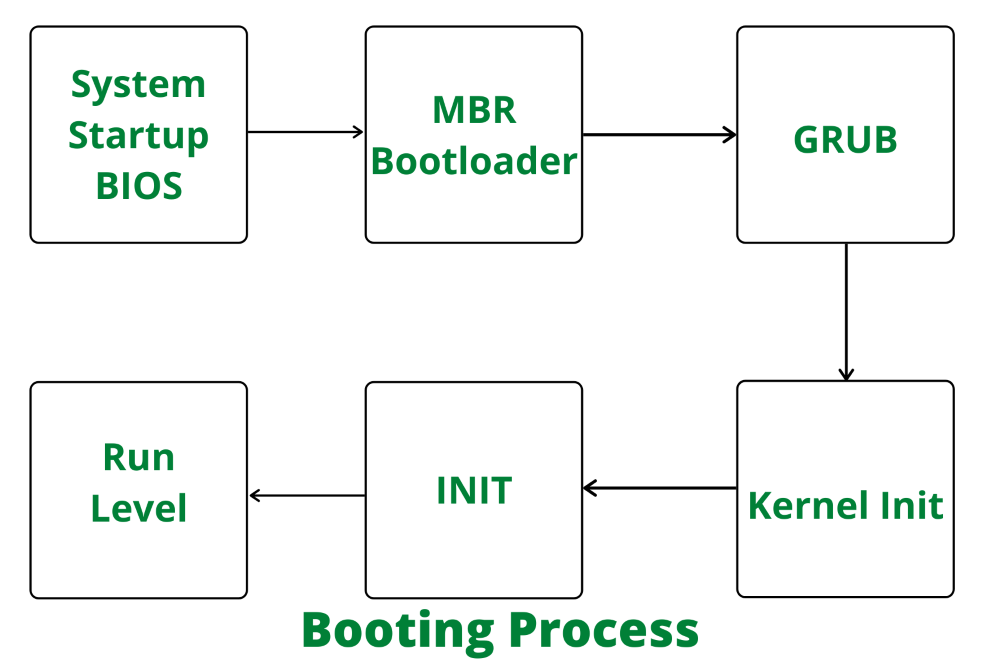
\includegraphics[width=0.75\textwidth]{Figure/07/1.png}
    \caption{Visualisasi proses booting komputer secara berurutan}
    \label{fig:m07-boot-sequence}
\end{figure}

Berdasarkan ilustrasi diagram pada Gambar \ref{fig:m07-boot-sequence}, tahapan \textit{booting} secara umum dapat dijabarkan menjadi 6 langkah sederhana:
\begin{enumerate}
    \item \textbf{System Startup BIOS}: Saat tombol \textit{power} ditekan, komputer akan menjalankan program bawaan mesin bernama BIOS. BIOS bertugas mengecek apakah komponen fisik (seperti RAM dan \textit{keyboard}) sudah berfungsi normal.
    \item \textbf{MBR Bootloader}: Setelah fisik dipastikan aman, BIOS akan mencari instruksi pertama di ujung memori penyimpanan (disk) yang lokasinya disebut MBR. MBR ibarat pintu masuk menuju program selanjutnya.
    \item \textbf{GRUB}: MBR kemudian memanggil program pengelola \textit{boot} yang lebih pintar, salah satunya adalah GRUB. GRUB inilah yang tahu persis di mana sistem operasi kita berada, lalu memuatnya ke memori utama (RAM).
    \item \textbf{Kernel Init}: Setelah dimuat ke RAM, inti dari sistem operasi (disebut \textit{Kernel}) mulai terbangun. Kernel secara resmi mengambil alih kendali komputer sepenuhnya dari tangan GRUB.
    \item \textbf{INIT}: Kernel kemudian menyalakan satu proses utama penggerak yang disebut \texttt{INIT}. Proses \texttt{INIT} inilah yang bertugas membangunkan fitur-fitur maupun layanan pendukung lain di dalam OS.
    \item \textbf{Run Level}: Ini adalah kondisi garis finis. Pada tahap \textit{Run Level}, komputer sudah "sadar" sepenuhnya (misalnya berhasil masuk ke layar Terminal/Desktop) dan siap menerima interaksi dari pengguna.
\end{enumerate}

\subsection{Kernel Bare-Bones dan Spesifikasi Multiboot}
Mengembangkan sistem operasi mensyaratkan kerangka dasar (\textit{bare-bones}) yang dapat beroperasi tanpa dukungan sistem operasi lain \cite{osdev_wiki_barebones}. Karena berstatus independen dan tidak menggunakan modul fungsi dari \textit{standard library}, inisialisasi awal pada perangkat keras komputer wajib diserahkan kepada komponen antarmuka yang sangat spesifik.

\subsubsection{Standar Multiboot pada Bootloader}
Agar perangkat \textit{bootloader} utama (seperti GRUB) bersedia menemukan dan memuat kernel spesifik OS ke dalam memori, kerangka OS didesain wajib mematuhi ketentuan dari \textbf{Spesifikasi Multiboot} (GNU). Berdasarkan spesifikasi instruksi ini, berkas kompilasi biner awal harus menyuntikkan deklarasi \textit{Multiboot Header} di bagian awal blok \textit{header} berkas (\textit{file format}). 

Tanda \textit{header} perizinan ini ditulis menggunakan bahasa Assembly (sebagaimana dideklarasikan melalui \texttt{boot.asm}) dengan menyertakan \textit{magic number} unik berbasis bilangan heksadesimal bernilai tetap (\texttt{0x1BADB002}) \cite{gnu_multiboot}. Kehadiran nomor ajaib ini menjadi patokan (\textit{signature}) identifikasi GRUB untuk mengenalinya sebagai OS terstandarisasi, sebelum perannya meredup dan mengandalkan proses siklus selanjutnya pada fungsi \texttt{main()} program bahasa terapan C (\texttt{kernel.c}).

\subsubsection{Manajemen Relokasi dengan Linker Script}
Pada arsitektur OS \textit{bare-metal}, penetapan perihal letak tatanan alamat memori tidak ditangani \textit{loader} dinamis. Ketiadaan itu mensyaratkan eksistensi berkas \textit{Linker Script} (\texttt{linker.ld}) untuk secara tegas mendikte alokasi perpindahan posisi kode memori \cite{bryant2015computer}. Pada sistem berbasis arsitektur x86, kernel OS umumnya diamanatkan agar diload ke ruang memori fisik minimal berawal di unit \texttt{1M} (\texttt{0x100000}), membiarkan ruang memori di bawah 1MB tetap diakses eksklusif sebagai alokasi sakral konfigurasi antarmuka untuk BIOS (\textit{Basic Input/Output System}) maupun Vesa-Graphic peranti tampilan visual perangkat.

\subsection{Simulasi Perangkat Keras melalui QEMU}
Setelah semua bagian kode dipersatukan menjadi satu format instalasi kepingan siap-boot (\texttt{os.iso}), eksekusi \textit{host-machine} pada komputer secara telanjang patut dihindari. Komputasi pengujian OS sangat sarat atas probabilitas kekacauan yang sanggup merusak alur partisi (*storage*) mesin \textit{host} sesungguhnya.

Keseluruhan perancangan diuji mutlak dalam isolasi peranti \textbf{QEMU}. Emulator x86 ini membentangkan platform simulasi lengkap mulai dari abstraksi CPU, register internal, kepingan Random Access Memory, hingga konfigurasi Serial-Port. Pemanfaatan QEMU menjadi prasyarat esensial guna mengekstrak pantauan alur \textit{log-sequence} operasi komputasi saat prosedur (\textit{Booting}) terjadi dari menit paling awal secara transparan, serta memudahkan rekam jejak apabila fungsi sinkronisasi (seperti penentuan jadwal \textit{task-scheduler}) menuai kecacatan algoritma teknis (*Crash-Faults*).

Tabel \ref{tab:m07-dasar-teori} merangkum hal-hal penting agar pembentukan konsep di atas lebih mudah ditinjau di modul ini.

\newpage
\begin{table}[!ht]
\caption{Tabel Ringkasan Dasar Teori}
\label{tab:m07-dasar-teori}
\centering
\begin{tabulary}{\textwidth}{|L|L|}
\hline
\textbf{Konsep / Tools} & \textbf{Penjelasan Singkat} \\ \hline
Bootloader (GRUB) & Program di sektor awal mesin yang membaca aturan GNU Multiboot dan membangunkan CPU arsitektur 32-bit. \\ \hline
\texttt{boot.asm} & Program instruksi mesin (\textit{Assembly}) bervolume hemat yang merengkuh (\textit{Entry-Point}) izin kendali booting OS. \\ \hline
Linker Script (\texttt{linker.ld}) & Merupakan set aturan logis tata letak posisi kode memori spesifik di RAM kernel (contoh blok: \texttt{0x100000}). \\ \hline
Multiboot Magic Number & Penanda (\textit{signature}) biner wajib penyuntingan GNU untuk menyatakan bahwa berkas bersangkutan diakui Bootloader. \\ \hline
QEMU & Sebuah perangkat lunak berbasis \textit{emulator} mandiri nan aman membedah pengujian alur OS instrumen format .iso. \\ \hline
\end{tabulary}
\end{table}

% --- 3. Alat dan Bahan ---
\newpage
\section{Alat dan Bahan}
\label{sec:m07-alat-bahan}

\subsection{Perangkat Keras}
\begin{itemize}
    \item PC atau Laptop dengan arsitektur prosesor x86/x64.
    \item Memori minimal 4GB RAM dan kapasitas penyimpanan sekunder yang memadai.
\end{itemize}

\subsection{Perangkat Lunak (Bahan Praktikum)}
\begin{itemize}
    \item Sistem operasi \textit{host} (Windows, Linux, atau macOS).
    \item Text Editor atau IDE (misalnya Visual Studio Code).
    \item Docker (Docker Desktop atau Docker Engine) untuk proses kompilasi (\textit{cross-compiling}) di lingkungan terisolasi.
    \item QEMU Emulator (khususnya paket \texttt{qemu-system-i386} atau \texttt{qemu-system-x86\_64}) sebagai mesin virtual.
    \item Paket kode dasar praktikum (\textit{Starter Code OS 32-bit}) yang dikloning/diunduh dari repositori GitHub: \url{https://github.com/Aziz097/starter-code-os32}.
\end{itemize}

% --- 4. Langkah-Langkah Praktikum ---
\newpage
\section{Langkah-Langkah Praktikum}

\subsection{Persiapan 1: Instalasi Dependensi Dasar dan Docker}
\label{sec:m07-persiapan-install}
Sebelum mengolah \textit{image}, Anda perlu memasang pustaka pengembangan (\textit{multilib compiler}, QEMU, dsb) serta \textit{engine} Docker di mesin \textit{host} utama Anda (khususnya untuk pengguna lingkungan basis distribusi Ubuntu/Debian).
\begin{enumerate}
    \item Buka Terminal dan perbarui indeks \textit{repository}, lalu pasang dependensi \textit{cross-compile} x86 dan QEMU:
    \begin{lstlisting}[language=bash, caption={Instalasi pustaka dasar dan perangkat virtual QEMU}]
sudo apt update
sudo apt install -y build-essential gcc-multilib nasm \
                    qemu-system-x86 grub-pc-bin xorriso
    \end{lstlisting}
    \item Selanjutnya, pastikan Docker terpasang di sistem. Jika belum, instal Docker Engine:
    \begin{lstlisting}[language=bash, caption={Instalasi Docker Engine}]
sudo apt install -y docker.io
    \end{lstlisting}
    \item (Opsional namun disarankan) Tambahkan \textit{user} Anda ke grup \texttt{docker} agar kelak terbebas dari awalan \texttt{sudo} ketika mengeksekusi komando Docker.
    \begin{lstlisting}[language=bash, caption={Konfigurasi hak otorisasi akses pengguna Docker}]
sudo usermod -aG docker $USER
    \end{lstlisting}
    \textit{Catatan: \textit{Restart} atau \textit{relog} Terminal Anda agar perubahan perizinan grup ini langsung terbaca.}
\end{enumerate}

\subsection{Persiapan 2: Menjalankan Mesin Terisolasi}
\label{sec:m07-persiapan-env}
Langkah ini menyiapkan ruang kerja terisolasi agar \textit{tools} kompilasi dan dependensi sistem operasi tidak mengotori mesin \textit{host} (laptop) Anda.
\begin{enumerate}
    \item Buka terminal, pastikan posisi Anda sudah berada di dalam folder proyek \texttt{starter-code-os32-main}, lalu terjun ke mode simulasi lingkungan dengan mengeksekusi \textit{script runner}-nya:
    \begin{lstlisting}[language=bash, caption={Perintah meluncurkan container Docker}]
# Di sistem Windows (menggunakan Git Bash/WSL) atau Linux/macOS:
./run-docker.sh
    \end{lstlisting}
    
    \begin{figure}[!ht]
        \centering
        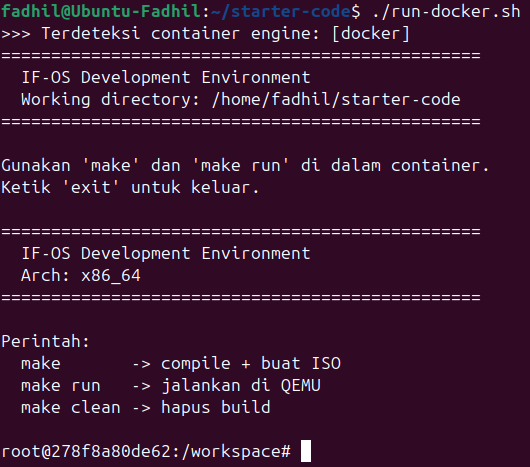
\includegraphics[width=0.85\textwidth]{Figure/07/8.png}
        \caption{Terminal masuk secara interaktif dengan indikator berpindahnya ruang kendali menjadi status \texttt{root@...:/workspace\#} di dalam kontainer \texttt{ifos-dev}}
        \label{fig:m07-docker-masuk}
    \end{figure}

    \item Skrip tersebut akan merakit atau menarik (\textit{pull}) peranti kontainer secara otomatis, ditandai dari tampilan baris \textit{working directory} Anda.
\end{enumerate}

\subsection{Sesi 1: Kompilasi Biner OS (Make)}
\label{sec:m07-sesi-1}
Di dalam lingkungan terisolasi ini, Anda akan menjahit (\textit{linking}) susunan berkas instruksi Assembly (\texttt{boot.asm}) dan C (\texttt{kernel.c}) menjadi satu \textit{file} instalasi terpadu (\texttt{os.iso}).
\begin{enumerate}
    \item Di dalam \textit{shell} kontainer Docker, periksa isi folder kerja menggunakan perintah \texttt{ls}. Secara mendasar, \textit{folder} ini adalah pantulan sikronisasi repositori Anda di mesin \textit{host} Anda.
    \item Lakukan kompilasi kode biner sumber dan menautkannya ke instruksi Multiboot GRUB melalui otomasi perintah sistem \texttt{make}:
    \begin{lstlisting}[language=bash, caption={Perintah kompilasi berkas instruksi OS}]
make
    \end{lstlisting}

    \begin{figure}[!ht]
        \centering
        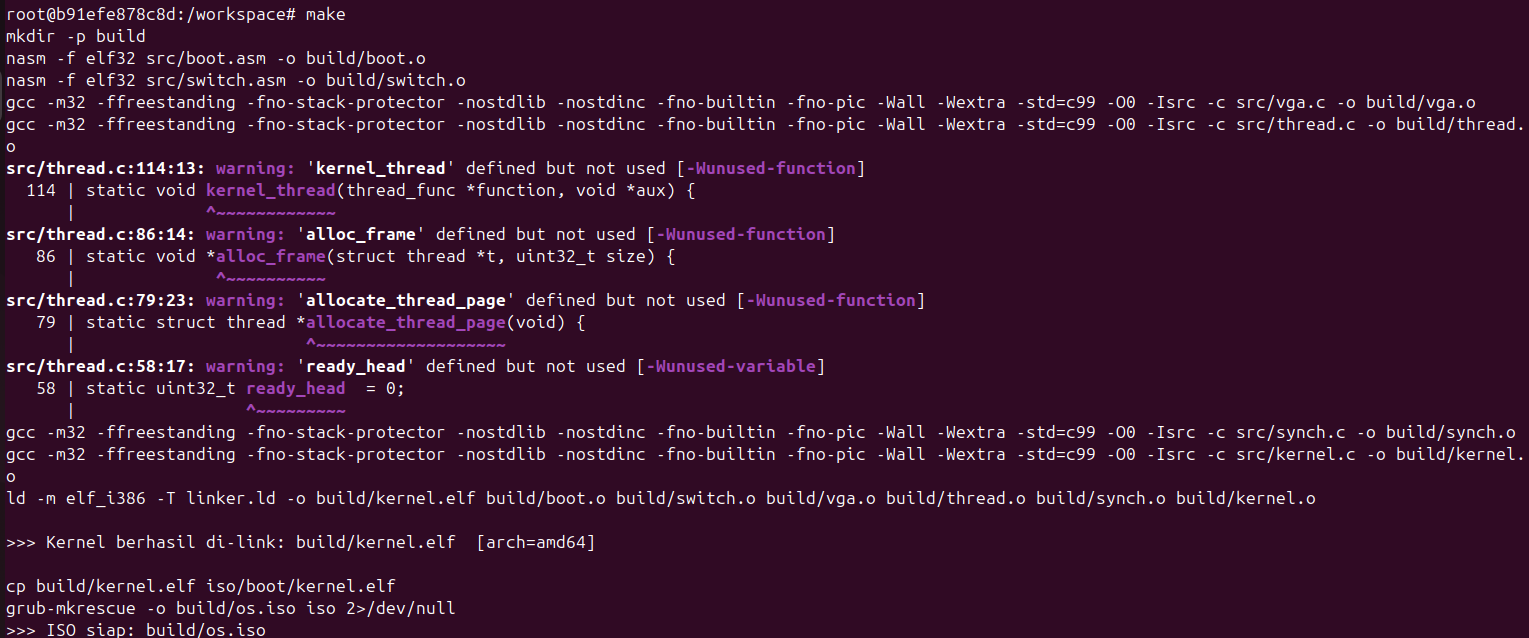
\includegraphics[width=0.9\textwidth]{Figure/07/9.png}
        \caption{Laporan suksesnya perintah \textit{make} pada \textit{shell} menautkan objek program C hingga \textit{linker} GRUB biner \texttt{os.iso}}
        \label{fig:m07-make-success}
    \end{figure}
    
    \item Perhatikan teks keluaran (\textit{output}) kompilator. Jika urutan berhasil, fungsi-fungsi instruksi selesai diproses dan Anda mendapat validasi bertuliskan: \texttt{>>> ISO siap: build/os.iso}.
\end{enumerate}

\subsection{Sesi 2: Eksekusi dan Verifikasi di QEMU}
\label{sec:m07-sesi-2}
Tahapan penutup modul ini adalah menguji coba berkas \textit{bare-metal} OS \texttt{.iso} tersebut ke dalam peranti simulator \textit{hardware} berarsitektur x86 bernama emulator QEMU.
\begin{enumerate}
    \item Keluar dari terminal kontainer Docker (dengan mengetik \texttt{exit}) atau buka jendela Terminal baru di mesin \textit{host} asli Anda. Pastikan posisi direktori Anda berada di folder proyek \texttt{starter-code-os32-main}.
    \item Laksanakan tes pembuka eksekusi skrip emulator dengan menjalankan perintah \textit{make} berikut di mesin \textit{host} Anda (yang sudah diinstal QEMU pada Persiapan 1):
    \begin{lstlisting}[language=bash, caption={Perintah memacu virtualisasi QEMU meluncurkan file OS biner}]
make run
    \end{lstlisting}

    \item Jendela layar QEMU (atau konsol emulator) akan muncul dan mengambil alih tampilan dengan antarmuka \textit{Bootloader} fiktif GRUB. \textit{Kernel loader} selanjutnya akan dipandu masuk melalui proses *booting* riil ke antarmuka utama sistem operasi.
    
    \item Oleh karena fitur fungsional komputasi \textit{Thread Scheduling} saat ini masih dirancang kosong secara alur \textit{stub} dalam struktur inti \textit{source code}, wajar apabila OS mencetak log luaran yang bermuara tertahan akibat pesan peringatan berikut (menandakan skema \textit{booting} sudah berhasil dimuat secara mulus):
    \begin{lstlisting}[caption={Pesan luaran *Thread block* sebagai bukti akhir keberhasilan simulasi di QEMU}]
===================================
  IF-OS  |  Praktikum Sistem Operasi
===================================

Inisialisasi sistem thread...
Membuat thread A, B, C...
Memulai scheduling...

ERROR: kernel_main() kembali dari thread_block()!
    \end{lstlisting}
\end{enumerate}
